%% This is an example first chapter.  You should put chapter/appendix that you
%% write into a separate file, and add a line \include{yourfilename} to
%% main.tex, where `yourfilename.tex' is the name of the chapter/appendix file.
%% You can process specific files by typing their names in at the 
%% \files=
%% prompt when you run the file main.tex through LaTeX.
\chapter{Reconstructed Objects}

The state-of-the-art CMS detector take a snapshot of each event and saves the detailed information of the collisions into datasets. In the datasets, we can access to event information with fully reconstructed objects including hits, tracks, muons, and vertex, which will be crucial for our data analysis to study B meson physics in heavy-ion collisions. Below, we will describe, in principle, how these objects with physical meaning are reconstructed from electronic signal in the CMS detector.

\section{Event}

As mentioned previously, an event is defined as a snapshot of one collision at the LHC. Many particles are produced in the collisions and then decay before they are detected in an event. Theoretically, to obtain the complete information of an event, we only need to know the position and momentum of each particle. Experimentally, we detect final state particles and record their kinematics. In high energy physics experiments, the particles reaching the detectors are $e^{\pm}$, $\mu^{\pm}$, $\pi^{\pm}$, $K^{\pm}$, $p$, $n$, $K^0_L$, $\gamma$. All other particles already decayed into these particles before they can be detected. In order to study them, they need to be reconstructed. Historically, this is used to be done by fast camera with high resolution. The Figure \ref{OmegaNick} shows a famous $\Omega^-$ baryon (Strangeness -3: $\Omega = sss$) event reconstructed from one of picture taken in the bubble chamber \cite{OmegaRef}.

\begin{figure}[hbtp]
\begin{center}
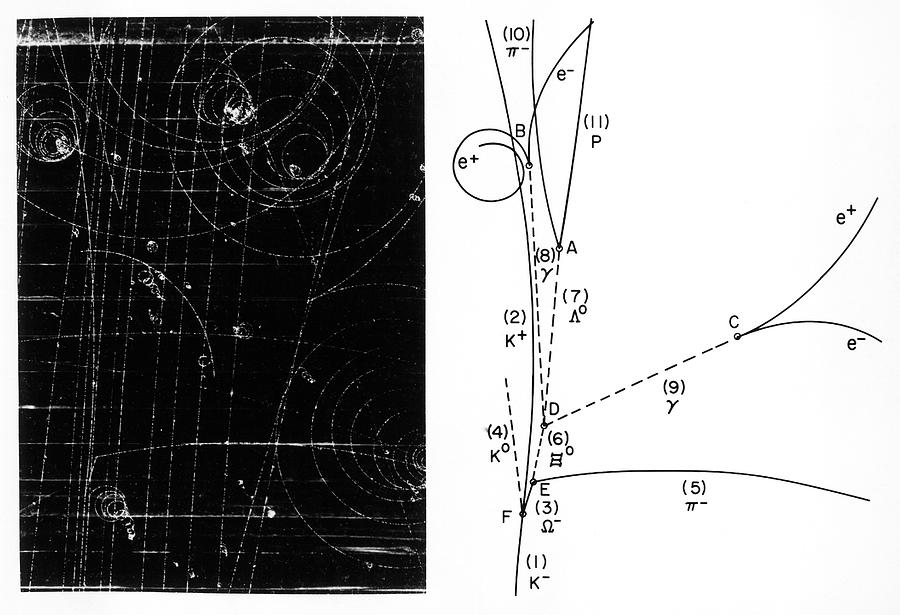
\includegraphics[width=0.70\textwidth]{Figures/Chapter4/Omega.jpg}
\caption{The bubble chamber picture of the an $\Omega^-$ baryon reconstructed from an event: $K^- p \rightarrow K^0 K^+ \Omega^- \rightarrow \Xi^0 \pi^- \rightarrow \Lambda^0 \gamma \gamma \rightarrow \pi^- p$ taken from the group led by Nicholas Samios at BNL is shown above.}
\label{OmegaNick}
\end{center}
\end{figure} 


Nowadays, the high speed electronics and semiconductor technologies have advanced. With the development of computing, detector hardware and readout electronics, high energy physics experiments are able to collect many events with higher precision of measurements. For instance, the CMS experiment has an event trigger rate of 100kHz, which corresponds to a rate of 100000 events per second with 100 GB/s information \cite{CMSDAQ}. Experimental data have become more digital and abstract instead of pictorial and intuitive. All events information is stored at a file format instead of a photograph. Physicists use computer to read the experimental data and develop software to perform analysis of each event, extract the physics information from the analysis, and interpret the physics results. 

In the following subsections, for simplicity, I will explain the reconstructed objects of events with only one charged particle. 

\section{Hit}

All reconstructed objects start from hits as the energy deposition of particle passing through the detectors. Here I will explain the concept of hits based on CMS silicon pixel tracker. Figure \ref{CMSPixChip}, the schematic view of a chip with silicon pixels in the CMS tracker


\begin{figure}[hbtp]
\begin{center}
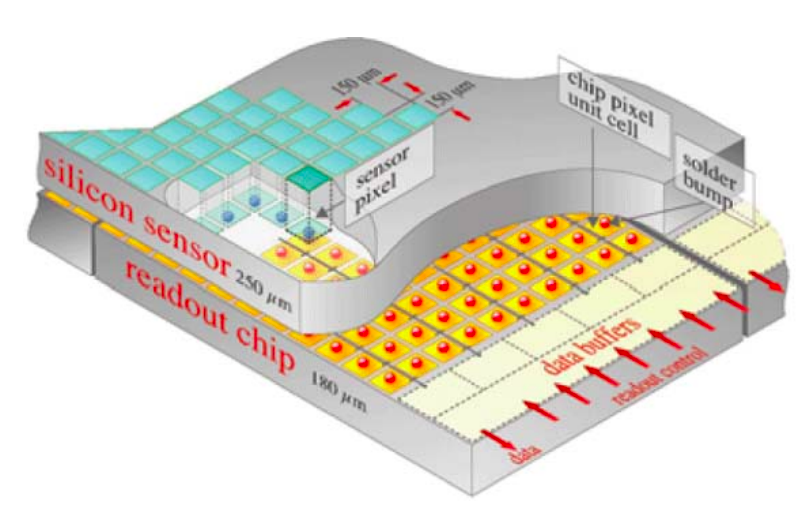
\includegraphics[width=0.50\textwidth]{Figures/Chapter4/CMSPixChip.png}
\caption{The schematic plot of a CMS silicon chip with pixel sensor is shown above.}
\label{CMSPixChip}
\end{center}
\end{figure} 

When a charged particle pass through a layer of the CMS silicon pixel detector, we can look at the charges collected by each pixel on that layer due to the ionization of electron-hole pairs by the high energy charged particle. Ideally, if a particle enter the tracker at a normal angle, only one pixel is fired. However, in reality, its neighboring pixels may also have some response. When the particle enter the tracker with a small angle  particularly when the part. Figure \ref{HitDemo} schematically demonstrates the firing pixel when a particle passing the layer

\begin{figure}[hbtp]
\begin{center}
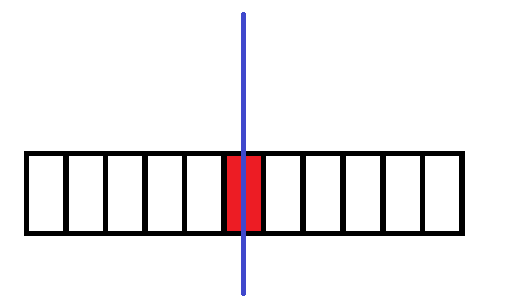
\includegraphics[width=0.48\textwidth]{Figures/Chapter4/Hit1.png}
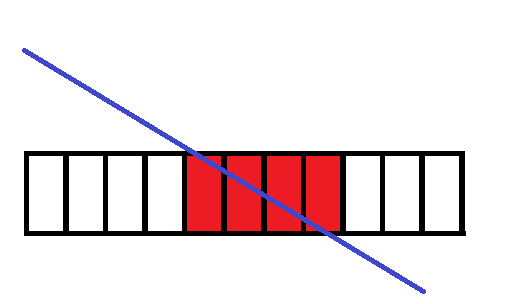
\includegraphics[width=0.48\textwidth]{Figures/Chapter4/Hit2.png}
\caption{The schematic views of a charged particle (blue line) entering the silicon pixel layer (black) at a normal angle (left) and a small tilting angle (right) with the pixels fired (red) are shown above. The left cluster has 1 hit and the right cluster has 4 hits.}
\label{HitDemo}
\end{center}
\end{figure} 

Here we call each firing pixel as a hit, which is demonstrated above in Figure \ref{HitDemo} in red. In CMS pixel tracker, the probability of a pixel firing when a charged particle passing through is greater than 99\% \cite{CMSTrackComp}, which means that it is very unlikely a hit is missing when a particle pass through the pixel. 



\section{Cluster}


Therefore, there should be at least one hit for each layer when a single particle pass through. We call the collection of the adjacent pixel hits in a layer due to one particle as a cluster \cite{CMSTrackComp}. Local hits reconstruction algorithm is implemented to obtain clusters. The number of electric charges $Q$ is associated to each hit. We can design an algorithm determine the center of a cluster according to the charges of each hit. A simple algorithm is to calculate the center of gravity of the cluster taking the weighted averaging of the charge and the position of each hit. In this case, for a cluster with a single hit, its position is simply the center of the pixel. For clusters with many hits, we develop a dedicated algorithm to estimate its position \cite{CMSTrackComp}. The position of a cluster is a measurement of the particle trajectory. 

However, in an event with many particles, the occupancy of each layer will be busy and the clusters will become complicated. The CMS collaboration develop  In CMS terminology, the conversion of electronic signal of pixels to clusters is called DIGI.


\section{Track}

\subsection{Overview of Basic Principles}

In a uniform external magnetic field, the trajectory of a charged particle will be a helix in 3 dimensions. Geometrically, five parameters are needed to parametrize a helix. A parametric curve of a helix moving in the Cartesian coordinates moving in the z direction is written as follows

\begin{equation}
x(t) = R \cos(\omega t) + a
\end{equation}

\begin{equation}
y(t) = R \sin(\omega t) + b
\end{equation}

\begin{equation}
z(t) = v t + c
\end{equation}

Therefore, we need at least 3 clusters to determine the all 5 parameters. 3 clusters can determine the radius $R$ and the center of the circle (a,b) and also can determine the straight line in the z-direction. Figure \ref{HelixAndFit} shows the helix path of a charged particle in a uniform magnetic field and the fit to determine the center and the radius of the helix.


\begin{figure}[hbtp]
\begin{center}
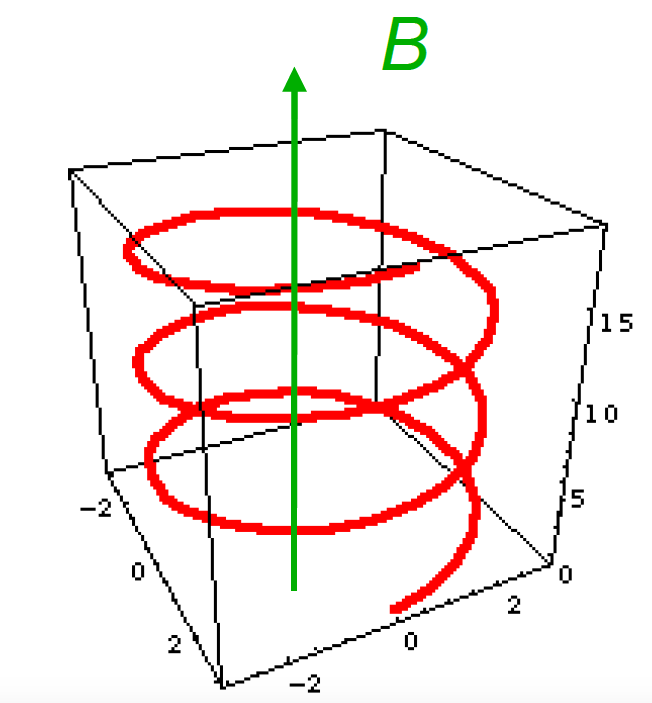
\includegraphics[width=0.35\textwidth]{Figures/Chapter4/Helix.png}
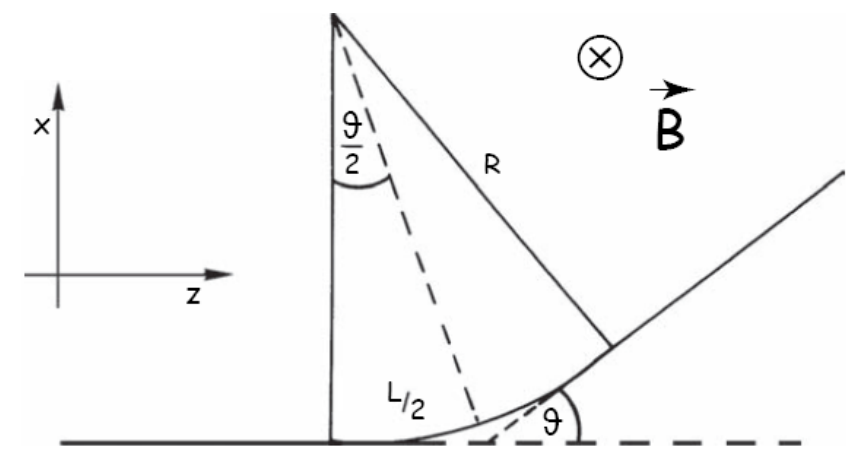
\includegraphics[width=0.55\textwidth]{Figures/Chapter4/FitToCircle.png}
\caption{The helix motion of a charged particle under a constant and uniform magnetic field $\vec{B}$ pointing in the +z direction (left) and the fit to 3 points to determine the center and the radius of a circle (right) are shown above.}
\label{HelixAndFit}
\end{center}
\end{figure} 

Moreover, we can determine transverse momentum of the charged particle according to the $R$ fitted from fit to the center of 3 clusters.

\begin{equation}
p_T  = qRB
\end{equation}

In general, the charges of the particles produced in the collision and pass through the tracker are $q = e$. Hence, $p_T = eRB$. For $p_T$ in the unit of GeV, $R$ in the unit of meter (m), and $B$ in the unit of tesla (T), we have 

\begin{equation}
p_T  \simeq 0.3 RB
\end{equation}

Therefore, as seen above from Figure \ref{HelixAndFit}, the transverse momentum resolution is driven by the determination of $R$ assuming we have a perfect measurement on the magnetic field $B$.

\begin{figure}[hbtp]
\begin{center}
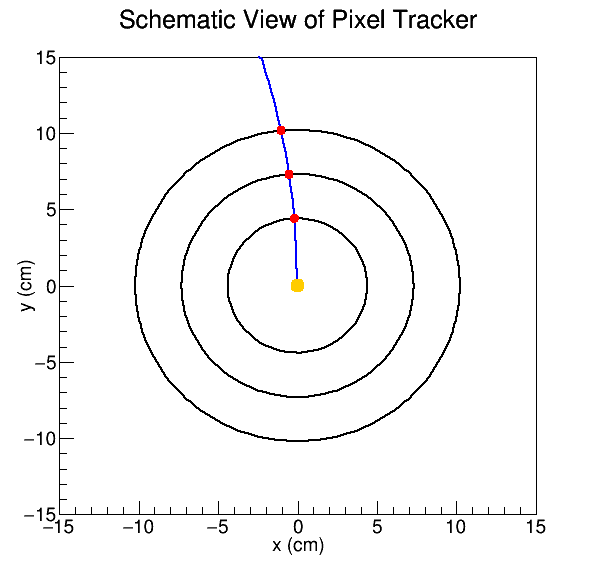
\includegraphics[width=0.45\textwidth]{Figures/Chapter4/PixLayTrk.png}
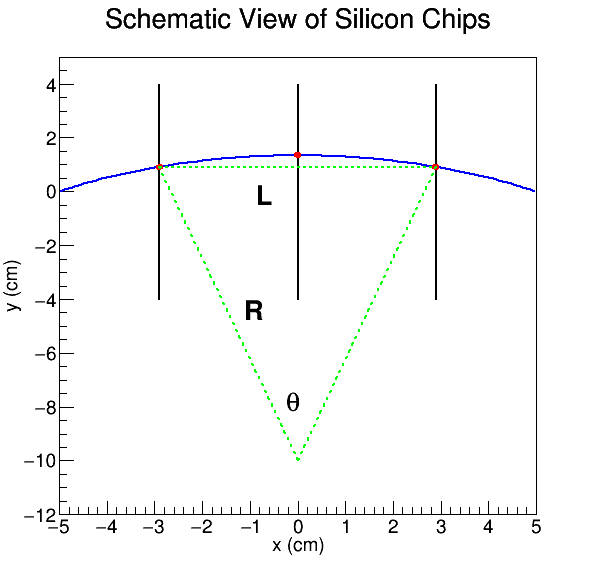
\includegraphics[width=0.45\textwidth]{Figures/Chapter4/FitOnHits.png}
\caption{A track (blue) initiated from the beam spot (orange) passing through 3 layers of pixel detectors (black) with 3 clusters (red) is shown on the left and the circular fit to the 3 clusters with the definition of $R$, $L$, and $\theta$ is shown on the right.}
\label{HelixAndFit}
\end{center}
\end{figure} 



According to Figure \ref{HelixAndFit} on the right, at high $p_T$, essentially in parallel, for a 3 cluster fit. In addition, we know that the layers in the pixel track has equal spacing $\Delta r$ between layers. For CMS pixel tracker, its inner most 3 layers has equal distance $\Delta r_{12} = \Delta_{23} =$ 2.9 cm \cite{CMSPIXInfo}. 


Hence, we can see that $L/2 = \Delta r$, which assume fixed with no uncertainties. Hence, we have

\begin{equation}
\frac{L}{2} = R \sin \frac{\theta}{2}
\end{equation}

Again, at high $p_T$, the angle $\theta$ will be very small since the radius of the circle $R >> \Delta r$, $\sin\theta \simeq \theta$ and $\cos\theta \simeq 1 - \frac{\theta^2}{2}$. Hence, we can use small angle approximation

\begin{equation}
L = 2 R \sin \frac{\theta}{2} \simeq R \theta
\end{equation}

Therefore,

\begin{equation}
p_T  \simeq 0.3 RB = 0.3 \frac{BL}{\theta}
\end{equation}


Hence, geometrically, we have


\begin{equation}
s = R - R \cos \frac{\theta}{2} = R (1 -  \cos \frac{\theta}{2}) =  R (1 -  \cos \frac{\theta}{2})  \simeq  \frac{L}{\theta} \{1 - [1 - \frac{1}{2} (\frac{\theta}{2})^2] \} =  \frac{L\theta}{8} = \frac{0.3BL^2}{8p_T}
\end{equation}

Thus, the uncertainties on both sides go as 

\begin{equation}
\sigma_s =  \frac{0.3BL^2}{8p_T^2} \sigma_{p_T}
\end{equation}

Hence, the transverse momentum resolution $\frac{\sigma_{p_T}}{p_T}$ is given by 


\begin{equation}
\frac{\sigma_{p_T}}{p_T} = \frac{8\sigma_s}{0.3BL^2} p_T
\end{equation}

Here, $\sigma_s$ is effective the position resolution of the silicon pixel detector. We can see that the transverse momentum resolution gets worse as $p_T$ increases in the high $p_T$ region. Figure \ref{CMSpTReso} shows the $\frac{\sigma_{p_T}}{p_T}$ as a function $p_T$


\begin{figure}[hbtp]
\begin{center}
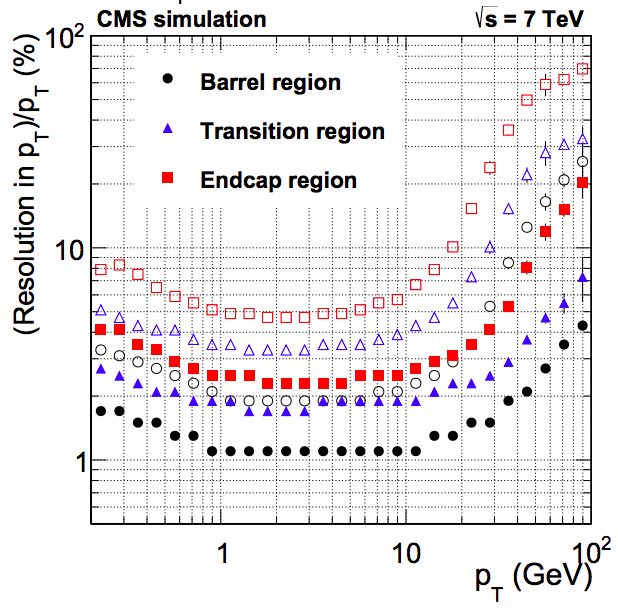
\includegraphics[width=0.60\textwidth]{Figures/Chapter4/CMSpTReso.png}
\caption{The transverse momentum resolution $\frac{\sigma_{p_T}}{p_T}$ of a track as a function of transverse momentum $p_T$ is shown above.}
\label{CMSpTReso}
\end{center}
\end{figure} 

We can see that a good agreement with linear growth of $\frac{\sigma_{p_T}}{p_T}$ for $p_T > 20$ GeV/c in the high $p_T$ region.

Longitudinally, $p_z$ can be determined by the $p_T$ and the angle $\Delta \theta$ in the transverse direction 

\begin{equation}
p_z = \frac{\Delta z}{\frac{R\Delta \theta}{p_T}} = 0.3B \frac{\Delta z}{\Delta \theta}
\end{equation}

At this point, we have obtain the trajectory with the complete kinematic information about a particle except its mass which will require particle identification in order to determine.

\subsection{CMS Tracking Algorithm}


Because the CMS silicon tracker has 3 pixel and 10 strip layers, a charge particle passing through all 13 layers should leave 13 clusters, which is much more than required to determine the helix. Moreover, in reality, collision events at the LHC, many tracks are produced at multiple vertices. In collider physics, we call use the concept of pileup events (PU), which is defined as events with more than one vertices. Figure \ref{CMSEvtInfo} shows the number of vertices and the number of tracks in $pp$ collisions at $\sqrt{s_{NN}} = $ 5.02 TeV

\begin{figure}[hbtp]
\begin{center}
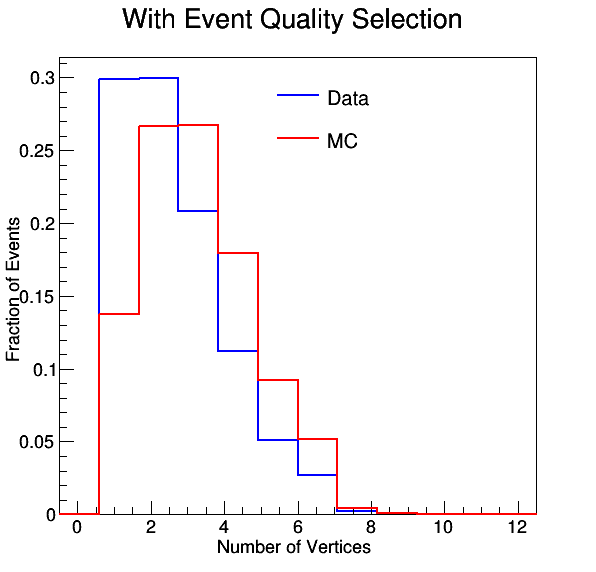
\includegraphics[width=0.48\textwidth]{Figures/Chapter4/Vertex.png}
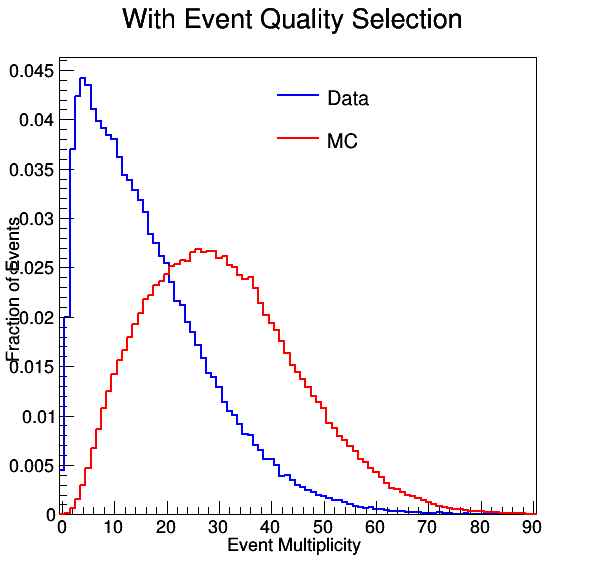
\includegraphics[width=0.48\textwidth]{Figures/Chapter4/Multiplicity.png}
\caption{The Data (blue) and MC (red) of the number of primary vertex distribution (left) and event multiplicity (right) are shown above. We can see that an event could be more than 1 vertices with more than 100 tracks, which make it very challenging to perform tracking.}
\label{CMSEvtInfo}
\end{center}
\end{figure} 

Hence, the CMS collaboration has developed the state-of-the-art tracking algorithm to reconstruct the paths and primary vertices of the collisions from the electronic readout signals. CMS tracking algorithm employs the Combinatorial Track Finder (CTF), an adaptation of the combinatorial Kalman filter \cite{CMSTrack1,CMSTrack2,CMSTrack3}, which in turn is an extension of the Kalman filter \cite{Kalman} to allow pattern recognition and track fitting to occur in the same framework. The collection of reconstructed tracks is produced by multiple passes (iterations) of the CTF track reconstruction sequence, in a process called iterative tracking \cite{CMSTrackComp}. The CMS tracking workflow and its performance are shown in Figure \ref{TrackWorkFlow} and Figure \ref{CMSTrackPer}



\begin{figure}[hbtp]
\begin{center}
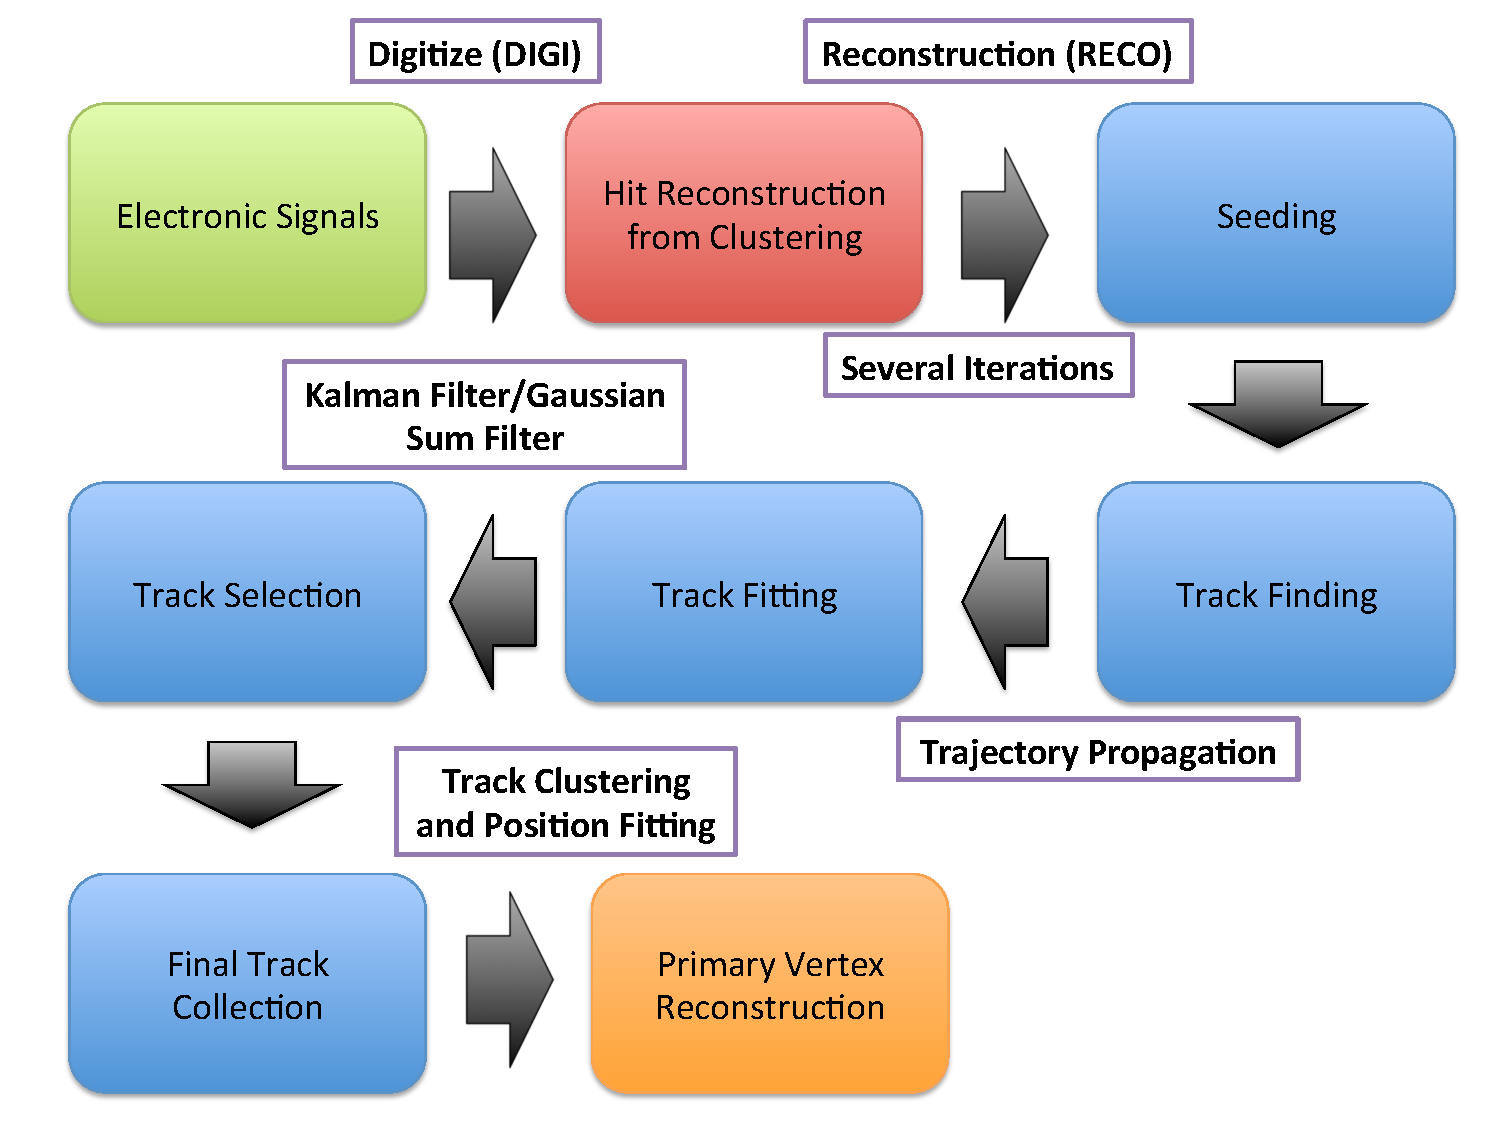
\includegraphics[width=0.90\textwidth]{Figures/Chapter4/TrackWF.pdf}
\caption{The schematic block diagram of CMS tracking workflow is shown above.}
\label{TrackWorkFlow}
\end{center}
\end{figure} 



\textbf{Track Seeding:} After obtain the clusters and reconstruct the hits, the tracking is in the track seeding stage. A dedicated seeding algorithm is designed to select the clusters, either a triplet or a pair, from the pixel layers and other combinations of pixel and strip layers before fitting \cite{CMSTrackComp}. After these steps, preliminary fits to the seeds named trajectory seeds are created.


\textbf{Track Finding:} Then, it moves on to the track finding stage. A six-step iteration process, which includes navigation, hit search, hit grouping, and trajectory update, is implemented with the application of CFT algorithms based on Kalman Filter to build track candidates. A schematic overview of the track finding process is shown below Figure \ref{CMSTrackFDWF}

\begin{figure}[hbtp]
\begin{center}
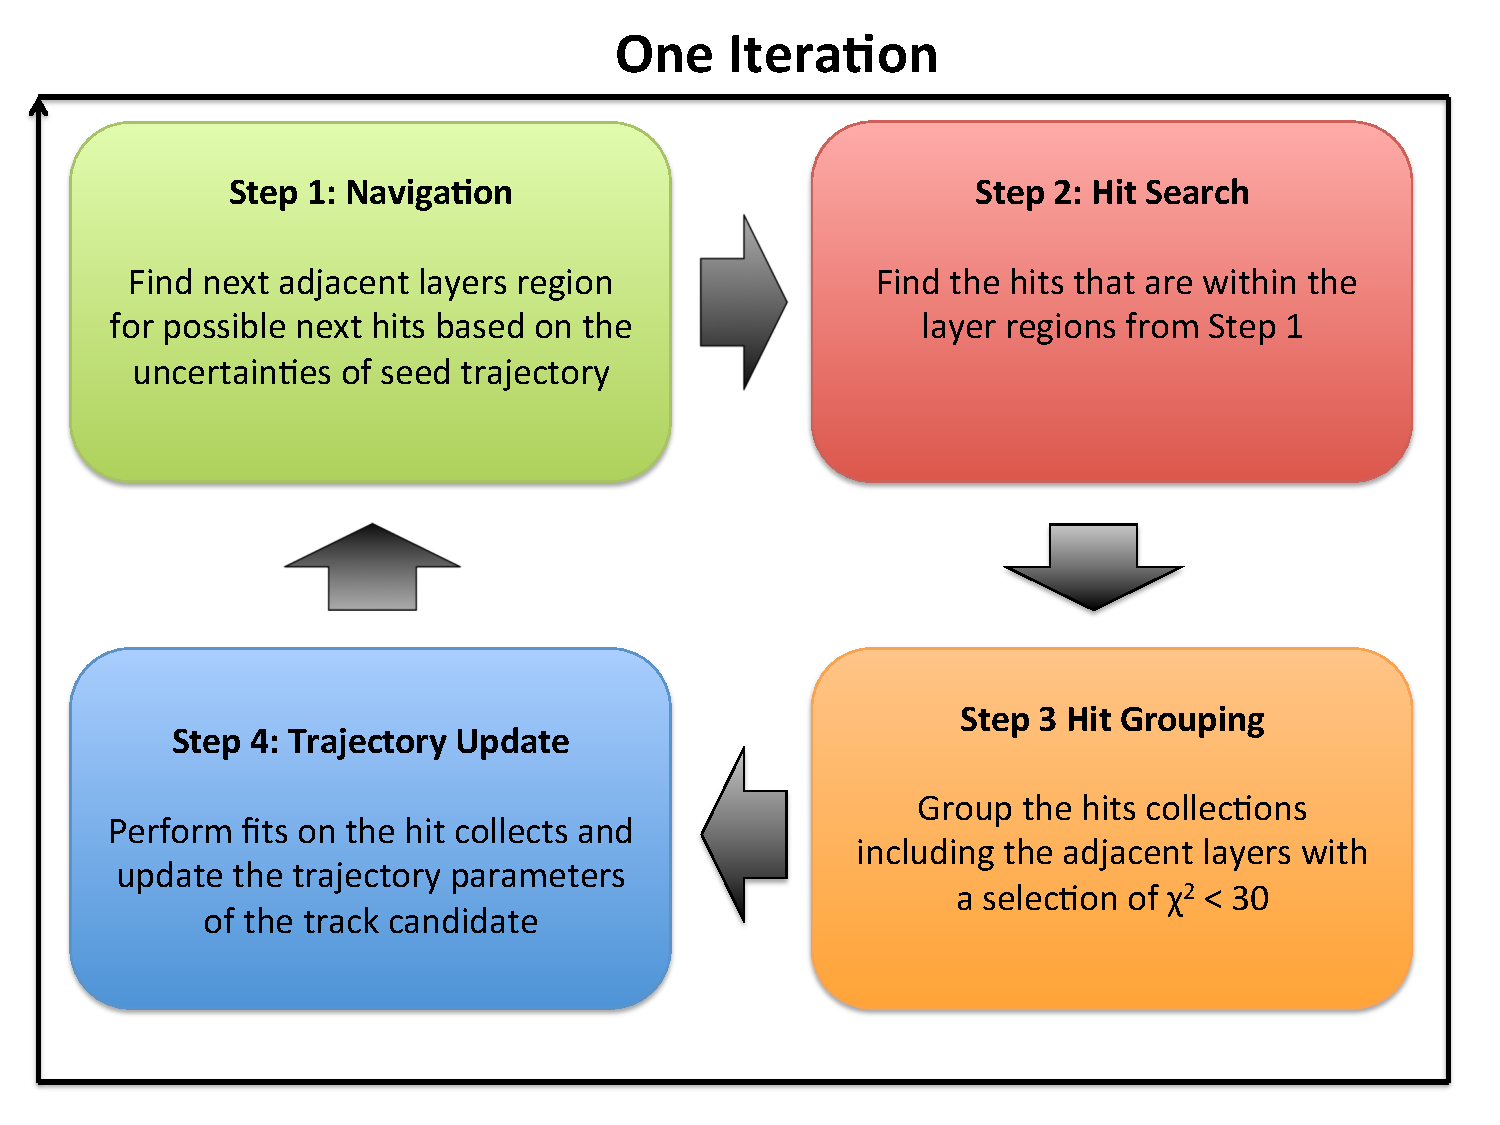
\includegraphics[width=0.900\textwidth]{Figures/Chapter4/TrackFDWF.pdf}
\caption{The four steps of CMS track finding workflow (left) and the schematic demonstration of each step (right) are shown above.}
\label{CMSTrackFDWF}
\end{center}
\end{figure} 


\begin{figure}[hbtp]
\begin{center}
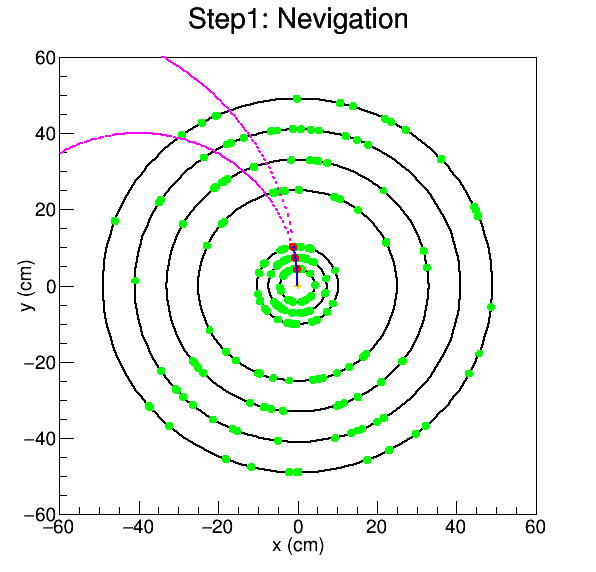
\includegraphics[width=0.48\textwidth]{Figures/Chapter4/Step1.png}
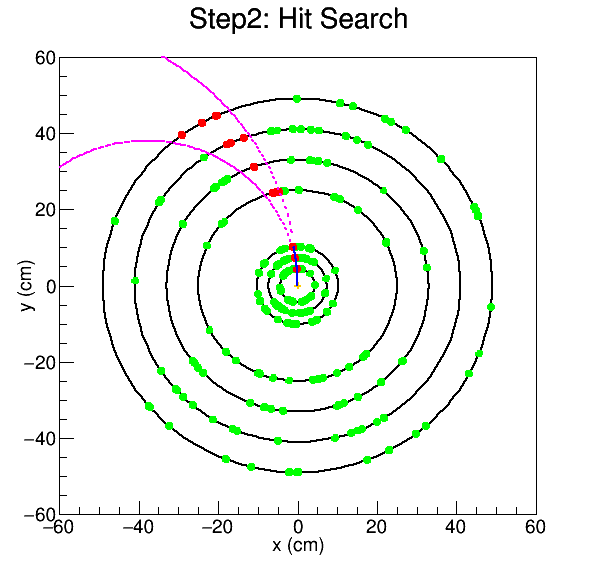
\includegraphics[width=0.48\textwidth]{Figures/Chapter4/Step2.png}
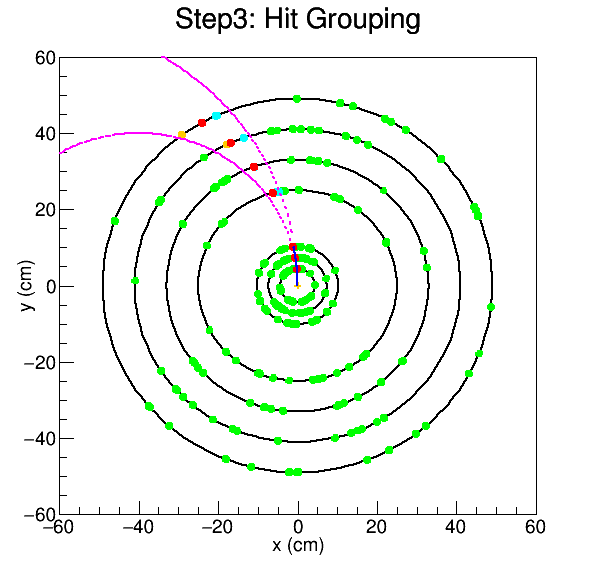
\includegraphics[width=0.48\textwidth]{Figures/Chapter4/Step3.png}
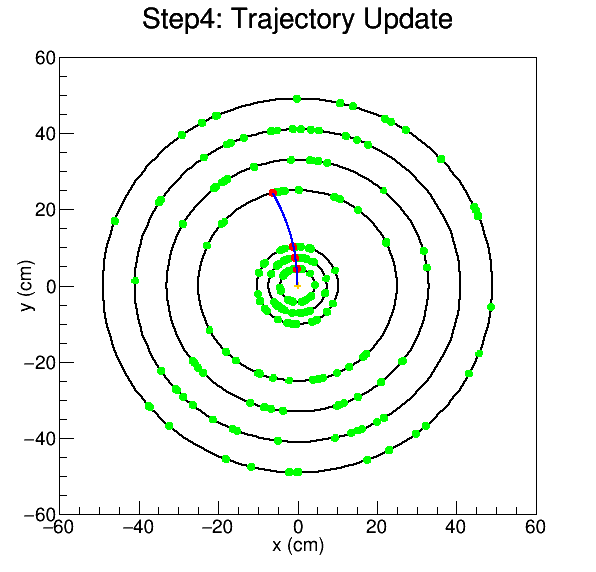
\includegraphics[width=0.48\textwidth]{Figures/Chapter4/Step4.png}
\caption{The four schematic plots demonstrating each of the four steps for track finding are shown respectfully above.}
\label{CMSTrackFDWF}
\end{center}
\end{figure} 

\textbf{Track Fitting:} Next, the tracking is in the stage of track fitting. Kalman filter \cite{Kalman} is applied to improve fitting performance. It starts from the innermost location with typically four hits \cite{CMSTrack1,CMSTrack2,CMSTrack3}. When extrapolating the trajectory from one hit to the next, the filtering and smoothing procedure is carried out with a Rugga-Katta propagator to obtain the best precision. $\chi^2 < $ 20 is required of each fit in order to improve its precision and reject fake tracks. Figure \ref{KalmanFitting} schematically shows how the Kalman filter fit along with Rugga-Katta propagator is applied in the iterative fitting algorithm for CMS tracking


\begin{figure}[hbtp]
\begin{center}
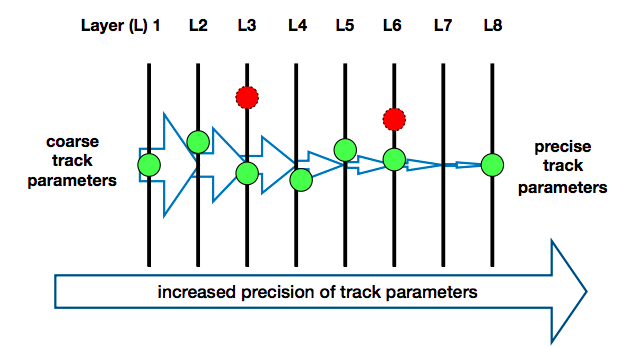
\includegraphics[width=0.80\textwidth]{Figures/Chapter4/KalmanFitting.png}
\caption{The schematic demonstration Kalman filter along with Rugga-Katta propagator to improve the tracks fitting is shown above.}
\label{KalmanFitting}
\end{center}
\end{figure} 


\textbf{Track Selection:} Subsequently, the tracking is in the stage of track selection. At this point, we have already obtained a preliminary track collection of one event. To improve the track quality and reject fake tracks, further selection based on the track properties will be applied. The following selection criteria are applied to select high quality tracks \cite{CMSTrackComp}

\begin{itemize}
\item Minimum number of layers in which the track has at least one associated hit
\item Minimum number of layers in which the track has an associated 3-D hit
\item Maximum number of layers that has no associate hits
\item $\chi^2/dof < \alpha_0 N_{layers}$ 
\item $|d_0^{BS}|/ \sigma_{d_0(p_T)} < (\alpha_1 N_{layers})^\beta$ 
\item $|z_0^{PV}|/ \sigma_{z_0(p_T,\eta)}  < (\alpha_2 N_{layers})^\beta$ 
\item $|d_0^{BS}|/\delta d_0 < (\alpha_3 N_{layers})^\beta$ 
\item $|z_0^{PV}|/\delta z_0 < (\alpha_4 N_{layers})^\beta$ 
\end{itemize}

Here, $\alpha_n$ and $\beta$ are configurable constant depend on the selection efficiency and purity requirements. $d_0^{BS}$ is the closest transverse distance of the track to the beam spot and $\delta d_0$ is its associated error. $z_0^{PV}$ is the distance along the beam-line from the closest pixel vertex and $\delta z_0^{PV}$ is its associated error. Hence, $|d_0^{BS}|/ \sigma_{d_0(p_T)}$ and $|z_0^{PV}|/ \sigma_{z_0(p_T,\eta)}$ are expressed in terms of significance. $\sigma_{d_0(p_T)}$ and $\sigma_{z_0(p_T,\eta)}$ are essentially the associated errors of $d_0^{BS}$ and $z_0^{PV}$ parametrized by track $p_T$ and $\eta$.


\textbf{Final Track Collection:}  Finally, after we apply the selections, we have obtained a final track collection for one event. Figure \ref{CMSTrackPer} shows the general performance of CMS tracking algorithm

\begin{figure}[hbtp]
\begin{center}
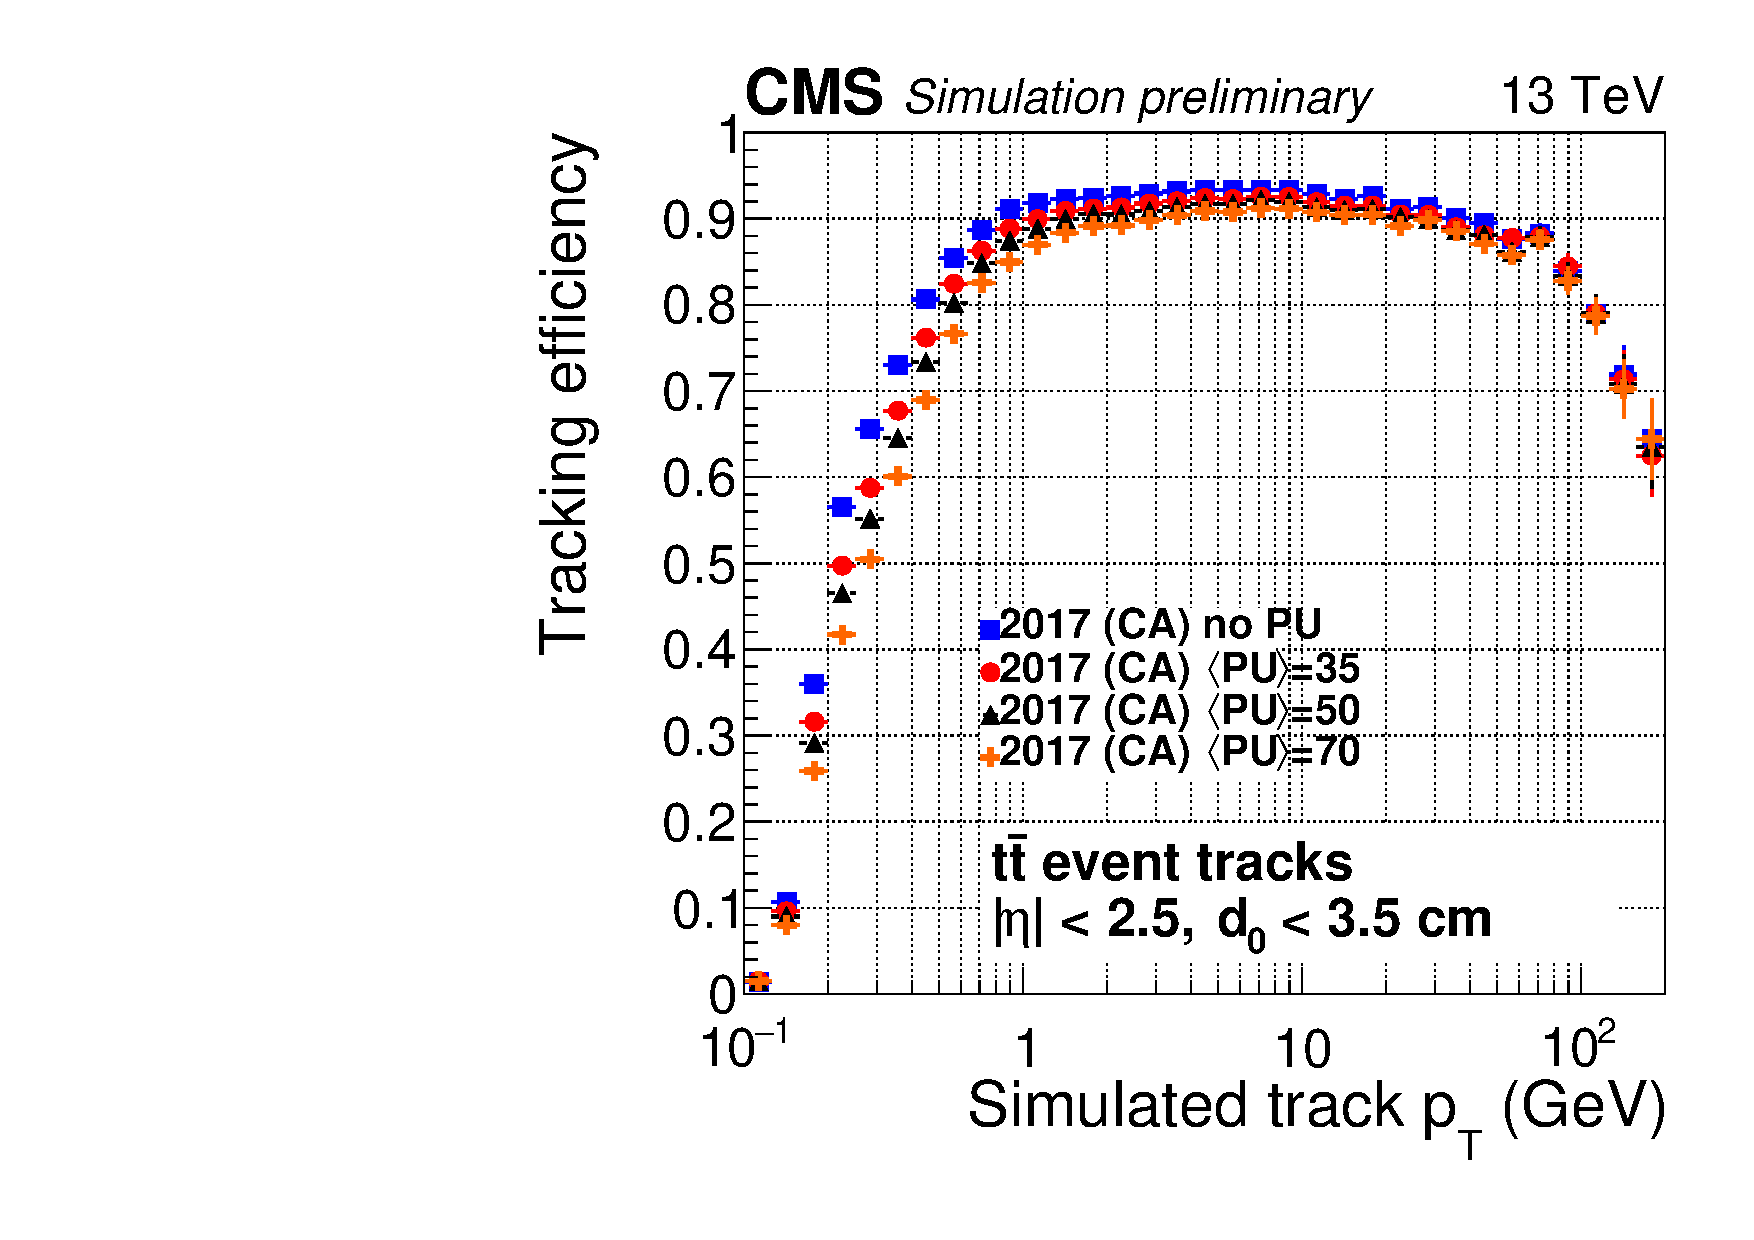
\includegraphics[width=0.48\textwidth]{Figures/Chapter4/TrackPTEff.pdf}
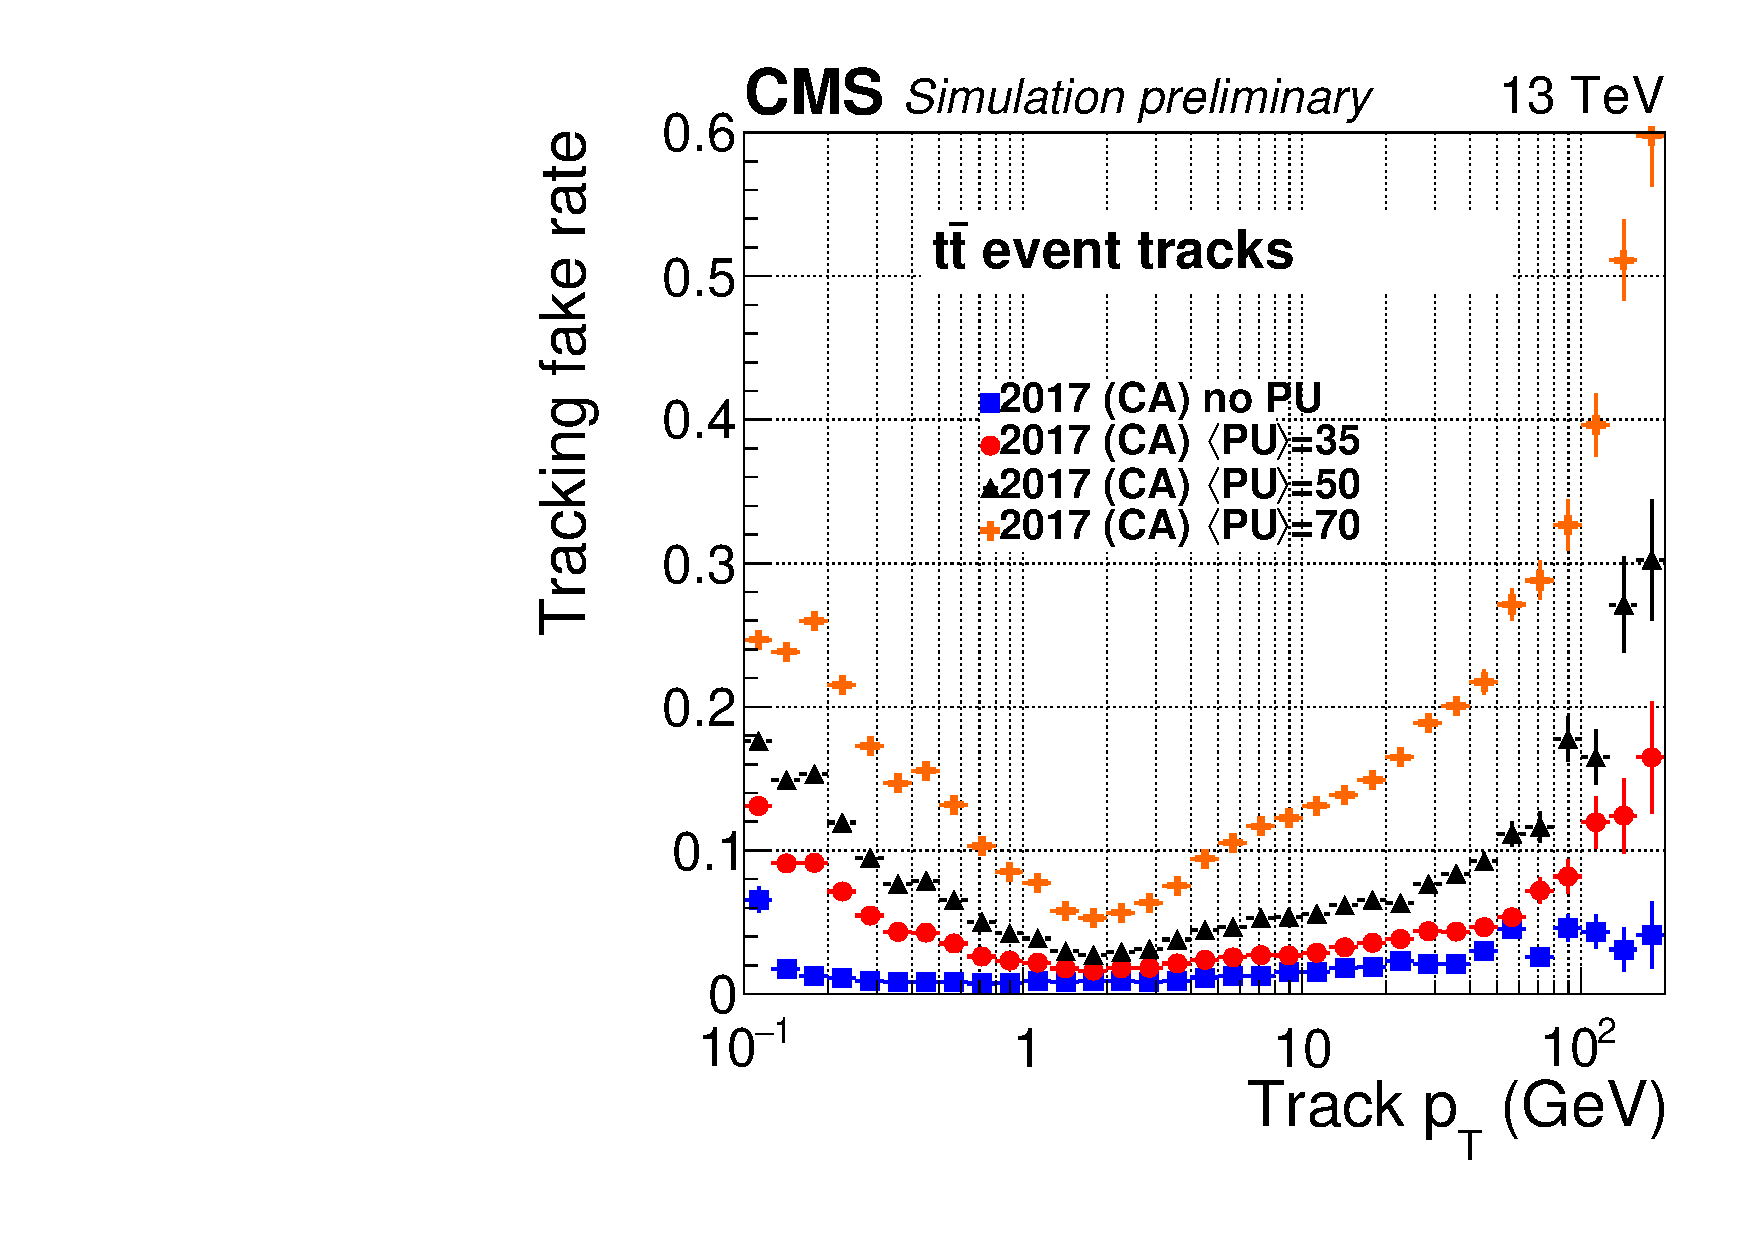
\includegraphics[width=0.48\textwidth]{Figures/Chapter4/TrackPTFake.pdf}
\caption{The CMS tracking efficiency (left) and fake rate (right) as a function of $p_T$ from simulations of $t \bar t$ events at 13 TeV with different pileup conditions are shown above.}
\label{CMSTrackPer}
\end{center}
\end{figure} 

We should note that a modified version of Kalman filter named Gaussian Sum Filter \cite{GSF} is applied to improve the tracking performance of electrons \cite{CMSTrackComp}.


\section{Muon}

The muon in the tracker uses an essentially the same tracking algorithms as other charged particles \cite{CMSTrackComp}. Tracking performance of muon is excellent. For isolated muons with 1 < $p_T$ < 100 GeV/c, the tracking efficiency is $>$ 99\% over the full $\eta$-range of tracker acceptance and does not significantly depend on $p_T$ while the fake rate is negligible \cite{CMSTrackComp}. We can require hits on the outer most muon chambers to identify muons because other charge particles will be stopped by the calorimeter and should not be able to enter the muon system as shown on Figure \ref{ParticleFlow}. The muon reconstruction workflow with the muon chambers are shown below in Figure \ref{MuonReco}


\begin{figure}[hbtp]
\begin{center}
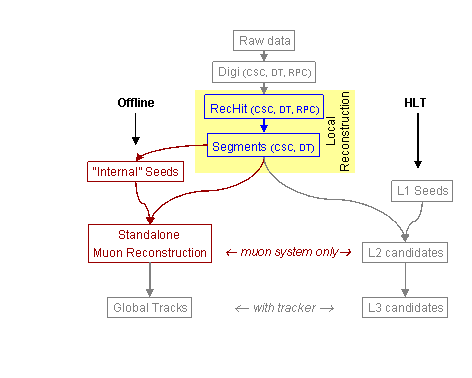
\includegraphics[width=0.65\textwidth]{Figures/Chapter4/MuonReco.png}
\caption{The schematic block diagram of muon reconstruction in the CMS muon system is shown above.}
\label{MuonReco}
\end{center}
\end{figure} 

In addition, since mouns also deposit some energy to the ECAL and HCAL, we can also access calorimeter information for the muons. Therefore, the CMS muon system has excellent capabilities of detecting, identifying, and reconstructing muons, which is crucial for heavy flavor physics studies. 

In CMS terminology, there are many types of muons based on their selection requirement in reconstruction. They are classified as follows:


\begin{itemize}
\item \textbf{Standalone Muons:} the muon segments reconstructed from muon chambers only.
\item \textbf{Tracker Muons:} the muon segments reconstructed from tracker only but also valid with the information from calorimeter and muon systems
\item \textbf{Global Muons:} the muons reconstructed from the fits on the hits of both trackering and muon systems
\item \textbf{RPC Muons:} the muons reconstructed with both inner tracker and the resistive plate detector only 
\item \textbf{Calorimeter-based Muons (Calo Muons):} the muons reconstructed with both inner tracker and calorimeters  
\end{itemize}

The relationship between stand alone muons, tracker muons, global muons, and calo muons are shown below in Figure \ref{MuonRel}

\begin{figure}[hbtp]
\begin{center}
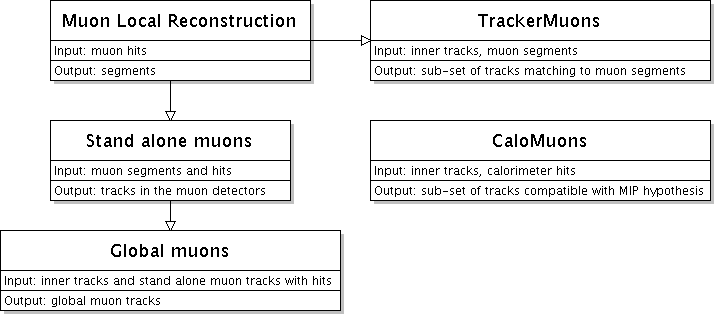
\includegraphics[width=0.75\textwidth]{Figures/Chapter4/MuonRel}
\caption{The relationship between different reconstructed muon in CMS is shown above}
\label{MuonRel}
\end{center}
\end{figure} 

For physics analysis, addition selections on muons including trigger, identification, and acceptance will be applied. We will further discussed them in the analysis chapter.

\section{Vertex}

In particle physics, the term vertex is similar to a vertex in Feynman diagram where old incoming particles are destroyed and new outgoing particles are created via an interaction at a space-time point. This has already shown in Figure \ref{OmegaNick} of the $\Omega^-$ baryon event where we can clearly see the vertices of $\Omega^-$ baryon creation and decay in the reconstructed plot on the right. 

\subsection{Primary Vertex}

By definition, in collider experiments, the primary vertex is assume where the hadron interact. Therefore, all particles produced in the collisions in that event originate from the primary vertices. With the final track collection for each event, assuming all the tracks are promptly produced at a given interaction point, we can determine the primary vertices by selecting the tracks, performing track clustering, and fitting for the position of each vertex using its associated tracks \cite{CMSTrackComp}. The selection criteria for the track to perform primary vertex are as follows:

\begin{itemize}
\item $|d_0^{BS}|/ \Delta d_0 < 5$
\item $N_{pixel} > 2$
\item $N_{strip} > 5$
\item $\chi^2/dof < 20$
\end{itemize}



The selection above make sure the tracks used have high quality and are indeed come from primary vertices. The deterministic annealing algorithm \cite{DAAlgo} is track clustering algorithm that CMS is currently using. An iterative process of minimize the annealing function of longitudinal distance between the tracks and the vertices gradual temperature reduction until dropping to the critical temperature is carried out to determine the number of vertices and their z coordinates \cite{CMSTrackComp}. A track can be used for more than one vertices during tracking clustering. Figure \ref{CMSEvtDisplay} is a $pp$ collision event display of the CMS detector with reconstructed tracks and primary vertices 

\begin{figure}[hbtp]
\begin{center}
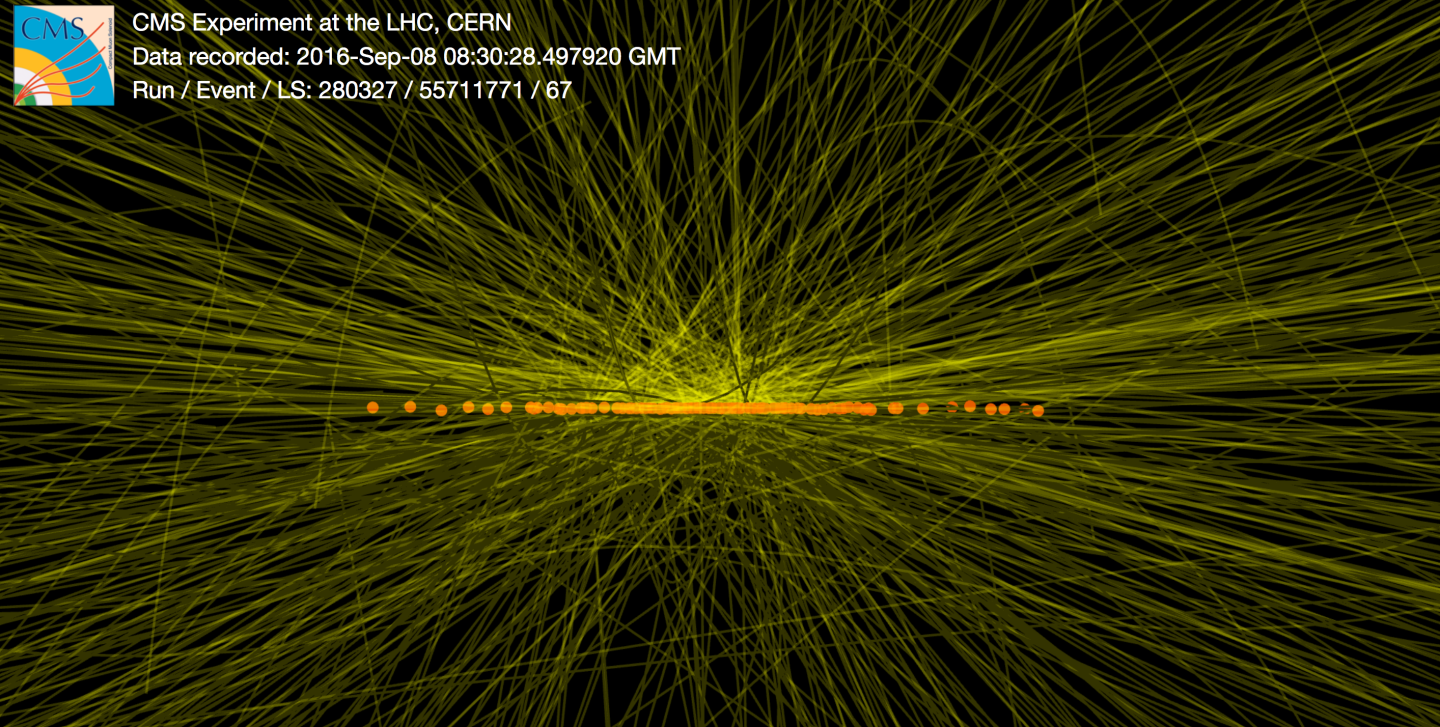
\includegraphics[width=0.85\textwidth]{Figures/Chapter4/CMSEvtDisplay.png}
\caption{A $pp$ collision event display of the CMS detector with reconstructed tracks (green curves) and primary vertices (yellow dots) is shown above.}
\label{CMSEvtDisplay}
\end{center}
\end{figure} 

\iffalse
Figure \ref{DAAlgoPlot} shows schematically the deterministic annealing algorithm


\begin{figure}[hbtp]
\begin{center}
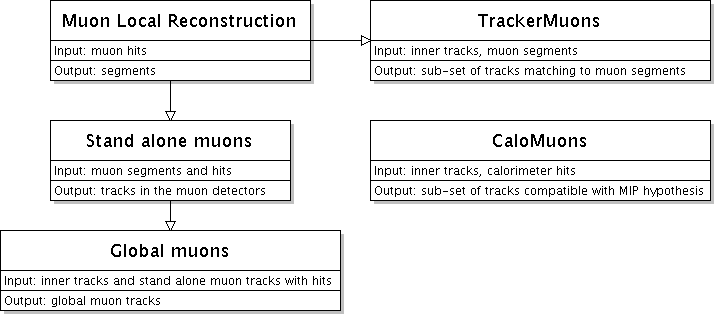
\includegraphics[width=0.75\textwidth]{Figures/Chapter4/MuonRel}
\caption{The relationship between different reconstructed muon in CMS is shown above}
\label{DAAlgoPlot}
\end{center}
\end{figure} 
\fi

After that, we have determined the vertex candidates with z coordinates. Then,  for the vertices candidates with at least two tracks, adaptive vertex fitter \cite{AVT} is applied to compute the best estimate of vertex parameters, including its x, y and z position, covariance matrix, and parameters characterizing the fitting performance such as the $\chi^2$, $n_{dof}$, vertex fitting probability, and the weights of the tracks used in the vertex. At this point we have obtain the complete information of an event with a final collection of tracks with best reconstructed vertices. The track and primary vertex information of each event will be saved in datasets for further physics analyses.

\subsection{Secondary Vertex}

Another object we should mention, particularly in the context of this thesis, is secondary vertex. Again, as seen from Figure \ref{OmegaNick}, there are many vertices in the $\Omega^-$ baryon event in its decay chain. We can the displaced vertex from the primary vertex due to the decay of a short-life particle produced at high energy as the secondary vertex. Figure \ref{D0Vtx} below is schematic plot of the decay topology of a prompt $D^0$ decay via the channel: $D^0 \rightarrow K^- \pi^+$ showing the primary vertex and secondary vertex  

\begin{figure}[hbtp]
\begin{center}
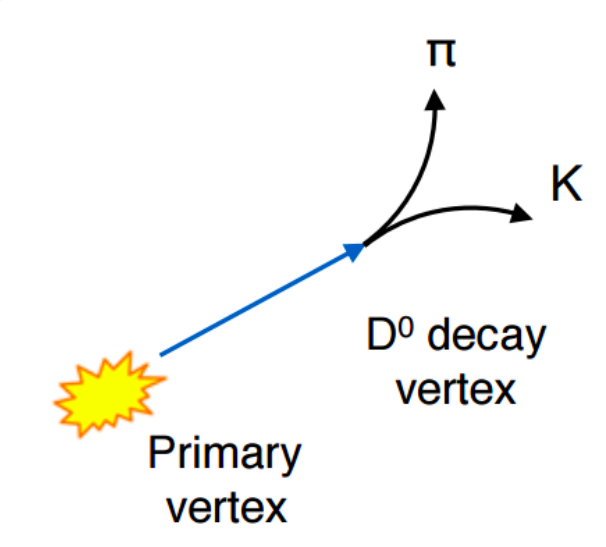
\includegraphics[width=0.45\textwidth]{Figures/Chapter4/D0Seconary.png}
\caption{The decay of $D^0 \rightarrow K^- \pi^+$ with the definition of secondary vertex is shown above}
\label{D0Vtx}
\end{center}
\end{figure} 

The decay length is defined as the distance between primary and secondary vertex. In LHC collisions, since the energy is very high, the particle produced from the primary vertex generally has a large momentum, which correspond to a large Lorentz gamma factor $\gamma \beta \simeq$ 5. For B mesons produced at the LHC, we estimate their length a $\gamma \beta c \tau \simeq 3$ mm due to its long lifetime $c \tau = 500$ $\mu$m \cite{AlphaTheoEx}. Therefore, the B meson secondary vertex is well seperated from the primary vertex and could even even viewed by eye. The relatively long B meson decay lengths make them ideal candidates to be fully reconstructed and study thanks to the excellent vertexing and tracking capabilities of the CMS detector.

Finally, we can also call the secondary vertex for a particle as the reconstructed mother particle's vertex. For instance, $B^0_s \rightarrow J/\psi \phi \rightarrow \mu^+\mu^- K^+K^-$. We can identify 3 secondary vertices. We call them $B^0_s$, $J/\psi$, and $\phi$ vertices. 

\iffalse

\section{Experimental Results}


Nevertheless, here I just take a simple case that only one charged particle is present in an event. In reality, LHC collision events in general have high pile with high multiplicity \cite{}. Figure \ref{} shows the number of reconstructed vertices in $pp$ collisions from MC and data. 


Therefore, when there are so many particles coming from many vertices in each event, the CMS Collaboration have designed more complicated algorithms to reconstruct events with physics objects mentioned above \cite{}.

\fi

